\documentclass[12pt, a4paper]{memoir}

% Essential packages
\usepackage[T1]{fontenc}
%%\usepackage[latin1]{inputenc}
\usepackage[french,english]{babel}

% personal packages
\usepackage [includehead, margin=1.5cm]{geometry}                % See geometry.pdf to learn the layout options. There are lots.
\usepackage{graphicx} % include images
\usepackage{hyperref} % urls, hyperlinks, etc
% \usepackage{pdfpages} % include pdf pages
\usepackage{enumitem} % customize itemize
\usepackage[backend=bibtex]{biblatex} % bibliography
\usepackage{csquotes} % Quote bibliography and add hyperlinks
% \usepackage{titlesec} % Modify chapter headings
% \usepackage{wrapfig} % wrap text around figures
% \usepackage{float} % force figure positions at the end of the file
\usepackage[linesnumbered,ruled,vlined]{algorithm2e}

% Packages from uga template
%\usepackage{fullpage}
\usepackage{mathptmx} % font = times
\usepackage{helvet} % font sf = helvetica
% \usepackage{amsmath}
% \usepackage{relsize}
% \usepackage{tikz}
% \usepackage{booktabs}
% \usepackage{textcomp}%textquotesingle
% \usepackage{multirow}
% \usepackage{pgfplots}

% \usetikzlibrary{arrows,shapes,positioning,shadows,trees}
% \makesavenoteenv{tabular}
% \makesavenoteenv{table}

\def\checkmark{\tikz\fill[scale=0.4](0,.35) -- (.25,0) -- (1,.7) -- (.25,.15) -- cycle;}

%Style des têtes de section, headings, chapitre
\headstyles{komalike}
\nouppercaseheads
\chapterstyle{dash}
\makeevenhead{headings}{\sffamily\thepage}{}{\sffamily\leftmark} 
\makeoddhead{headings}{\sffamily\rightmark}{}{\sffamily\thepage}
\makeoddfoot{plain}{}{}{} % Pages chapitre. 
\makeheadrule{headings}{\textwidth}{\normalrulethickness}
%\renewcommand{\leftmark}{\thechapter ---}
\renewcommand{\chaptername}{\relax}
\renewcommand{\chaptitlefont}{ \sffamily\bfseries \LARGE}
\renewcommand{\chapnumfont}{ \sffamily\bfseries \LARGE}
\setsecnumdepth{subsection}
\addbibresource{biblio.bib}

% Customize itemize item markers
\renewcommand\labelitemi{-}

% Add source to figures caption
\newcommand*{\captionsource}[2]{%
    \caption[{#1}]{%
        #1%
        \\\hspace{\linewidth}%
	\textbf{Source:} \textit{#2}%
    }%
}

% Some settings for the title page
%\titleformat{\chapter}[display]{\normalfont\huge\bfseries}{}{0pt}{\Huge}
%\titlespacing*{\chapter} {0pt}{20pt}{40pt}

% Force footnotes to stay on one page
\interfootnotelinepenalty=10000

% Title page formatting -- do not change!
\newcommand{\HRule}{\rule{\linewidth}{0.5mm}}
\pretitle{\HUGE\sffamily \bfseries\begin{center}\HRule \\[0.2cm]} 
	\posttitle{\end{center}\HRule}
\preauthor{\LARGE  \sffamily \bfseries\begin{center}}
\postauthor{\par\end{center}}
\newcommand{\jury}[1]{% 
\gdef\juryB{#1}} 
\newcommand{\juryB}{} 
\newcommand{\session}[1]{% 
\gdef\sessionB{#1}} 
\newcommand{\sessionB}{} 
\newcommand{\option}[1]{% 
\gdef\optionB{#1}} 
\newcommand{\optionB} {}

\renewcommand{\maketitlehookd}{% 
\vfill{}  \large\par\noindent  
\begin{center}\juryB \bigskip\sessionB\end{center}
\vspace{-1.5cm}}
\renewcommand{\maketitlehooka}{% 
	\vspace{-1.5cm}\noindent
\includegraphics[height=10ex]{./imgs/uga-logo.png}\hfill
\includegraphics[height=10ex]{./imgs/ryax-logo.png}\hfill
\includegraphics[height=10ex]{./imgs/Logo-LIG.jpg}\hfill
\includegraphics[height=12ex]{./imgs/ENSIMAG.png}
\bigskip
\begin{center} \large
Master of Science in Informatics at Grenoble \\
Master Informatique \\ 
Specialization \optionB  \end{center}\vfill}
% =======================End of title page formatting

\option{MoSIG} 
\title{Simulation of a Kubernetes Cluster with Validation in Real Conditions} %\\\vspace{-1ex}\rule{10ex}{0.5pt} \\sub-title} 
\author{LARUE Théo}
\date{Defense Date, 2020} % Delete this line to display the current date
\jury{
	Research project performed at Laboratoire d'Informatique de Grenoble \\\medskip
Under the supervision of:\\
Michael Mercier\\\medskip
Defended before a jury composed of:\\
Head of the jury\\
Jury member 1\\
Jury member 2\\
}
\session{September \hfill 2020}
\setcounter{tocdepth}{4}
\setcounter{secnumdepth}{4}

\begin{document}
\selectlanguage{english} % french si rapport en français
\frontmatter
\begin{titlingpage}
\maketitle
\end{titlingpage}

%\small
\setlength{\parskip}{-1pt plus 1pt}

\renewcommand{\abstracttextfont}{\normalfont}
\abstractintoc
\begin{abstract} 
	TODO : rework this with the new intro


	The rise of containerized applications has provided web platforms with
	much more control over their resources than they had before with their
	physical servers. Soon enough, developers realized they could go even
	further by automating container management operations to allow for even
	more scalability. The Cloud Native Computing Foundation was founded in
	this context, and developed Kubernetes which is a piece of software
	capable of container orchestration, or in other words, container
	management. Now, as we observe a convergence between HPC (High
	Performance Computing) and the Big Data field where Kubernetes is
	already the standard for some applications such as Machine Learning,
	discussions about leveraging containers for HPC applications rose and
	interest in Kubernetes has grown in the HPC community. One of the many
	challenges the HPC world has to face is scheduling, which is the act of
	allocating tasks submitted by users on available resources. In order to
	properly evaluate and develop schedulers researchers have used
	simulators for decades to avoid running experiments in real conditions,
	which is costly both in time and resources. However, such simulators do
	not exist for Kubernetes or are not open to the public. While the
	default scheduler works great for most of the Cloud Native
	infrastructures Kubernetes was designed for, some teams of researchers
	would rather be able to experiment with different batch processing
	policies on Kubernetes as they do with traditional HPC. Our goal in
	this master thesis is to describe how we developed Batkube, which it is
	an interface between Kubernetes schedulers and Batsim, a general
	purpose infrastructure simulator based on the Simgrid framework and
	developed at the LIG.

\end{abstract}
\abstractintoc

\renewcommand\abstractname{Acknowledgement}
\begin{abstract}
I would like to express my sincere gratitude to .. for his invaluable assistance and comments in reviewing this report... 
Good luck :) 
\end{abstract}

\renewcommand\abstractname{R\'esum\'e}
\begin{abstract} \selectlanguage{french}
	Abstract mais en franchais
\end{abstract}
\selectlanguage{english}

\tableofcontents* % the asterisk means that the table of contents itself isn't put into the ToC
\normalsize

\mainmatter
\SingleSpace

\chapter{Introduction}

The need for scalable computing infrastructure has increased tremendously in
the last decades. Nearly every field of computer science, from research to the
service industry, now needs a proper infrastructure and by 2025, computation
technology could reach a fourth of the global electricity
spending\cite{andrae2017total}.  Even the public sector is now in need for
efficient distributed infrastructure as the concept of smart cities is
developing.

Organizations generally know what type of infrastructure will meet their needs.
It can take the form of Big Data centers to store and analyze data,
High-Performance Computers for computing intensive tasks or GPU banks for
machine learning or crypto-currency mining.  However, studying those
infrastructures extensively is much more challenging.  As these computers reach
scales in the order of warehouses\cite{barroso2018datacenter}, quantifying a
system's performance under varying loads, applications, scheduling policies and
system size quickly becomes undoable without expensive real world experiments.
In fact, the nature of scheduling problems\cite{scheduler-complexity} alone
make theoretical studies hard.  This is an issue for organizations as they rely
on thoses studies to determine the size of the required system or choose
optimal scheduling
policies.\\

Simulation allows to tackle these issues by enabling users to draw conclusions
empirically without the need to fire up real workloads. Indeed, running an
entire experimental campaign on a real system represents consequencial costs
both in time and money. With simulation, The gain in both time and spent energy
can be extreme : a HPC job spanning months on a real system can be resolved in
a matter of minutes on any domestic computer.  Another major point is that it
also brings reproducibility to these experiments, that otherwise would have to
be run on the exact same systems as their first iteration. With simulation, one
can recreate the same conditions for any experiment anywhere they want, and
expect the same results.\\

However, simulations need to be run with sound models for the results to be
exploitable and in that regard, simulators usually fall under several
pitfalls\cite{poquet:tel-01757245}. Very often simulators are implemented at
the same time as new schedulers or Resource and Jobs Management
Systems\footnote{The RJMS is the software at the core of the cluster. It is a
synonym for a scheduler and manages resources, energy consumption, users' jobs
life-cycle and implements scheduling policies.} in order to validate their
algorithms. Thus, they are strongly coupled together and are not usable with
any other software. They are either shipped with the software itself or worst,
they are never released and discarded at the end of the development process.
Moreover, still according to \cite{poquet:tel-01757245}, strong coupling may
lead to unrealistic models. In that case cluster resources can be accessed with
ease by the scheduler, resulting in it having very precise information about the
system state to take its decisions.  This conflicts with the real world as a
scheduler may not have access to all the information it wants, or may suffer
from latency when getting it from the system.\\

To try and assess these issues a team of researchers at the LIG developed
Batsim\cite{dutot:hal-01333471} which is a general purpose infrastructure
simulator with modularity and separation of concerns in mind. Batsim is based
on SimGrid\cite{casanova:hal-01017319} which is a framework for developing
simulators for distributed computer systems. Simgrid is now a 20 years old
framework that has been used in many
projects\footnote{https://simgrid.org/usages.html}, making it a sound choice to
run scalable and accurate models of the reality.

Batsim was designed to support algorithms written in any languages, as long as
they support its communication protocol. It means that, while any scheduler
found in the wild can potentially be run on a Batsim simulation, they still
have to be adapted to make them compatible. This master's project is dedicated
on developing an interface between Batsim and
Kubernetes\footnote{https://github.com/kubernetes/kubernetes/} schedulers in
order to run Kubernetes clusters simulations. Kube\footnote{Another term to
designate Kubernetes. It is also sometimes called k8s.} is an open source
container management software widely exploited in the industry for its ease of
use and wide range of capabilities. It has freed developers from the cumbersome
task of setting up low level software infrastructure on their servers and
automates maintenance, scaling and administration of their applications. For
all these reasons it has become a de-facto solution for any organization that
wishes to build new internet platforms from the ground up.\\

TODO : what we where able to do (summary of the simulator capabilities,
experimentations, results)

%\subsection{A bit of context : High Performance Computing}
%
%TODO
%
%A general definition of HPC would be :
%``\textit{High Performance Computing (HPC) most generally refers to the
%		practice of aggregating computing power in a way that delivers
%		much higher performance than one could get out of a typical
%		desktop computer in order to solve large problems in science,
%		engineering, or
%		business.}
%\footnote{\url{https://wwwen.uni.lu/university/high_performance_computing}}''.
%HPC can either refer to ``High Performance Computing'' or ``High Performance
%Computer'' but it is generally clear which one it refers to, given the
%context.
%
%A HPC workload is composed of numerous tasks hungry for computational resources
%which are executed in parallel on different machines (that we can refer to as
%compute resources or nodes). These tasks may be completely independant like
%when different users each submit a single task, or they may also be tightly
%coupled together as when a single user submits a job that is composed of
%several tasks than can be run in parallel. In that case, the whole system
%becomes very sensitive to latency as these tasks have got to communicate
%together. This is done through MPIs (Message Passing Interfaces) which
%represent a large part of the HPC field.\\

\chapter{State of the art}

\section{Why simulation?}

\chapter{Implementation}
\section{The scheduling problem}
\begin{displayquote}[][]
	\textbf{schedule} \textit{n.} : A plan for
	performing work or achieving an objective, specifying the order and
	allotted time for each part.
\end{displayquote}

In a general way, scheduling is the concept of allocating available resources
to a set of tasks, organizing them in time and space (the resource space). The
resources can be of any nature, and the tasks independent from each others or
linked together.

In computing the definition remains the same, but with automation in mind.
Schedulers are algorithms that take as an input either a pre-defined workload,
which is a set of jobs  to be executed - the tasks are called jobs in this
context -, or simple jobs submitted over time by users in an unpredictable
manner. In the latter case, the jobs are added to a queue managed by the
scheduler. Scheduling is also called batch scheduling or batch processing, as
schedulers allocate batches of jobs at a time. Jobs are allocated on machines,
virtual or physical, with the intent of minimizing the total execution time,
equally distributing resources, minimizing wait time for the user or reducing
energy costs. As these objectives often contradict themselves, schedulers have
to implement compromises or focus on what the user really needs or requires.  

The scheduler has many factors to keep in mind while trying to be as efficient
as possible, such as :

\begin{itemize}
	\item Resource availability and jobs resource requirements
	\item Link between jobs (some are executed in parallel and need synchronization, some are independent)
	\item Latency between compute resources
	\item Compute resources failures
	\item Jobs priority
	\item Machine shutdowns and restarts
	\item Data locality
\end{itemize}

All these elements make scheduling a very intricate problem that is at best
polynomial in complexity, and often NP-hard\cite{scheduler-complexity}.
Moreover, with the growing complexity of modern RJMS and the wide variety in infrastructures, scheduler
performances are rather unpredictable.

\section{SimGrid}
\section{Batsim}

\section{Kubernetes}
\subsection*{Kubernetes overview}
In the early stages of application development, organizations used to run their
services on physical servers. With this direct approach came many challenges
that needed to be coped with manually like resources allocation,
maintainability or scalability. In an attempt to automate this process
developers started using virtual machines which enabled them to run their
services regardless of physical infrastructure while having a better control
over resources allocation.  This led to the concept of containers which takes
the idea of encapsulated applications further.

%\begin{figure}[h]
%	\centering
%	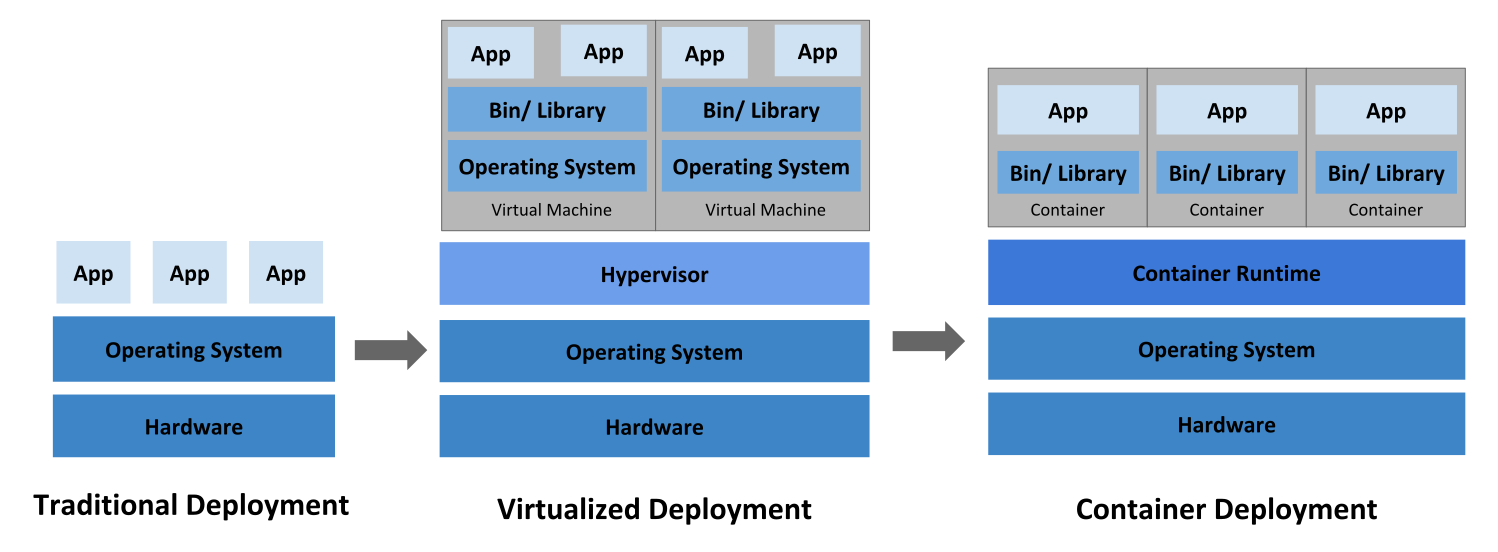
\includegraphics[width=\textwidth]{./imgs/container_evolution.png}
%	\captionsource{Evolution of application deployment.}{https://kubernetes.io/docs/concepts/overview/what-is-kubernetes/}
%	\label{fig:container-evolution}
%\end{figure}

Containers can be thought of as lightweight virtual machines. Unlike the
latter, containers share the same kernel with the host machine but still allow
for a very controlled environment to run applications. There are many
benefits to this : separating the development from deployment, portability,
easy resource allocation, breaking large services into smaller micro-services
or support of continuous integration tools (containers greatly facilitate
integration tests).\\

The CNCF\footnote{\url{https://www.cncf.io/}} (Cloud Native Computing
Foundation) was founded in the intent of leveraging the container technology
for an overall better web. In a general way, we now speak of these
containerized and modular applications as cloud native computing :

\textit{``Cloud native technologies empower organizations to build and run
	scalable applications in modern, dynamic environments such as public,
	private, and hybrid clouds. Containers, service meshes, microservices,
	immutable infrastructure, and declarative APIs exemplify this
	approach.}

\textit{These techniques enable loosely coupled systems that
	are resilient, manageable, and observable.  Combined with robust
	automation, they allow engineers to make high-impact changes frequently
	and predictably with minimal toil.``}\footnote{\url{https://github.com/cncf/toc/blob/master/DEFINITION.md}}

Kubernetes\footnote{\url{https://kubernetes.io/}} is the implementation of this
general idea and was anounced at the same time as the CNCF. It aims at
automating of the process of deploying, maintaining and scaling containerized
applications. It is industry grade and is now the de-facto solution for
container orchestration.

The basic processing unit of Kubernetes is called a \textbf{pod} which is
composed of one or several containers and volumes\footnote{A volume is some
	storage space on the host machine that can be linked to containers, so
	they can read persistent information or store data in the long term}.
In the cloud native context a pod most often hosts a service or micro-service.

\begin{figure}[h]
	\centering
	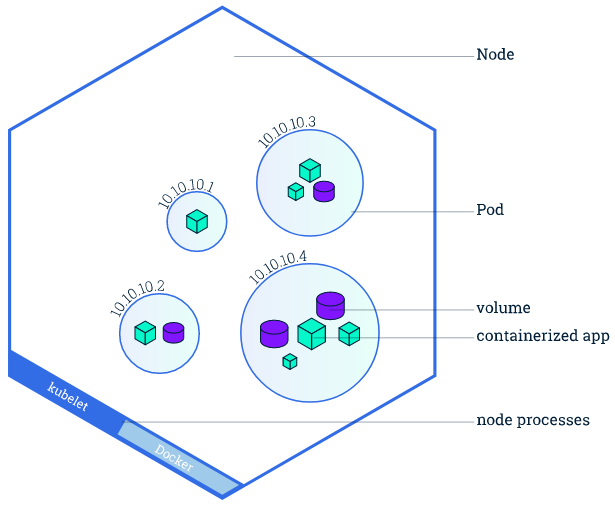
\includegraphics[scale=0.5]{./imgs/node-overview.png}
	\captionsource{Node overview}{https://kubernetes.io/docs/tutorials/kubernetes-basics/explore/explore-intro/}
	\label{fig:node-overview}
\end{figure}

Pods are bundled together in \textbf{nodes} (figure \ref{fig:node-overview})
which are either physical or virtual machines. They represent another barrier
to pass through to access the outside world which can be useful to add layers
of security or facilitate communication between pods. Nodes take the idea of
containerisation further by encapsulating the already encapsulated services.
Each node runs at least one pod and also one \textbf{kubelet} which is a
process responsible for communicating with the rest of Kubernetes (or more
precisely, with the master node which in turns communicates with the api
server). A set of nodes is called a \textbf{cluster}. Each Kubernetes instance
is responsible for running a cluster.

Kubernetes revolves its API server which is its central component (figure
\ref{fig:kube-components}). The majority of operations between components go
through this REST API like user interactions through kubectl or scheduling
operations.

\begin{figure}[h]
	\centering
	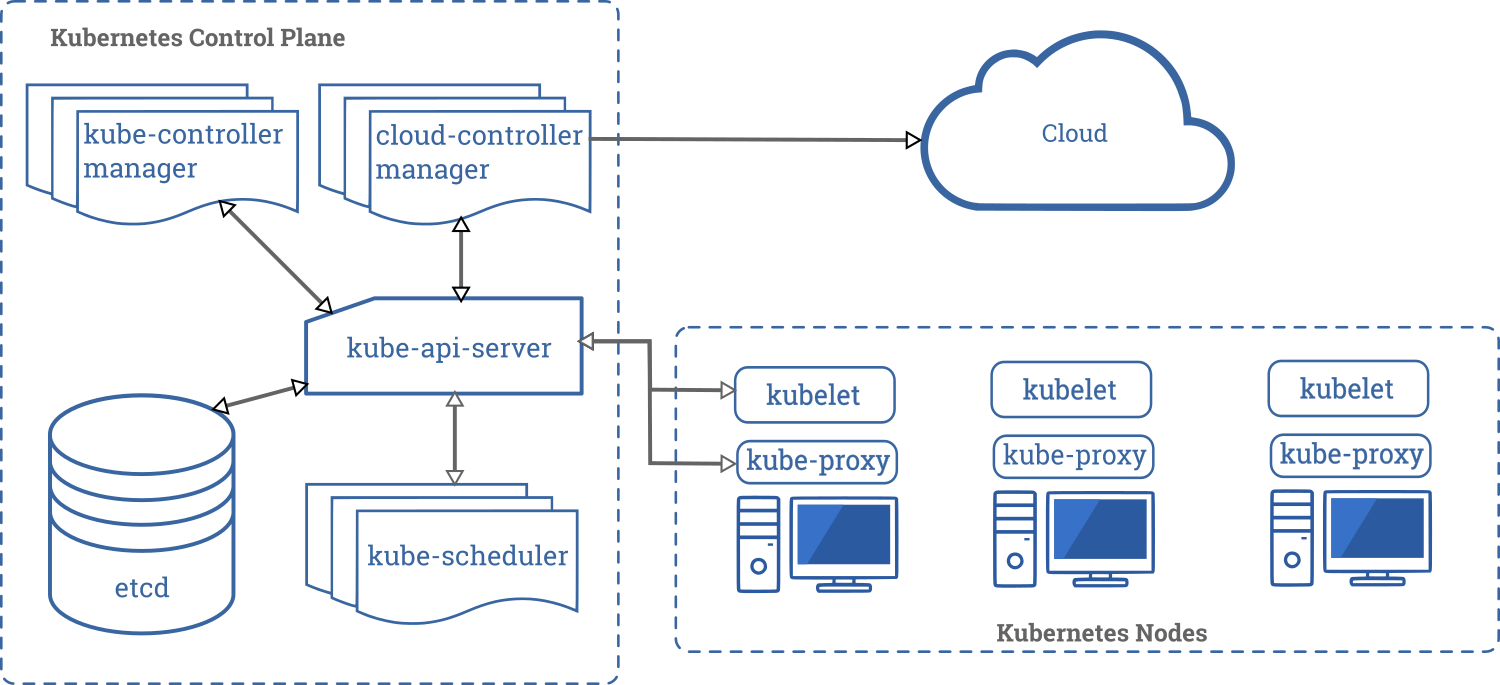
\includegraphics[width=\textwidth]{./imgs/components-of-kubernetes.png}
	\captionsource{Components of Kubernetes}{https://kubernetes.io/docs/concepts/overview/components/}
	\label{fig:kube-components}
\end{figure}

\newpage % hotfix for problematic figure placement
\subsection*{HPC and Kubernetes}
The difference between HPC and Cloud Native computing lies in the workloads
they are intended to tackle.  Kubernetes was designed for Cloud Native
applications. Services or micro services are run in containers and are expected
to be available at all times : they are replicated as many times as the user
desires and restarted whenever a failure occurs. High availability is at the
core of Kubernetes container management.  On the other hand, depending on
scheduling policies, HPC is focused on user wait time, maximizing resource
usage, optimizing energy costs... For instance, in case of failure, it is
sometimes not sufficient to restart the single job that failed : the entire
submission must be re-run if it is part of several jobs computed in parallel.

Kubernetes is now the standard for AI and Machine Learning as shown by the many
efforts at making this coupling an efficient
environment\cite{lee2017design}\cite{233001}\cite{10.1145/3154842.3154845},
which brought an increasing interest for container driven HPC aswell and
Kubernetes for HPC in particular. Batch schedulers such as
kube-batch\footnote{\url{https://github.com/kubernetes-sigs/kube-batch}} have
been implemented for kube, and numerous HPC applications like
slurm\footnote{\url{https://slurm.schedmd.com/containers.html}} now support containers as well.

Indeed, containers have many advantages that HPC users can benefit from. Here
are some notable ones:
\begin{itemize}
	\item First off, research has shown that Kuberenetes offer similar
		performance to more standard bare metal HPC\cite{8950981}.
	\item Users will get the same environment everywhere making up for a
		uniform and standardized workplace.
	\item Portability : users could seamlessly hop from one infrastructure
		to another based on their needs and criteria like price,
		performance, and capabilities rather than compatibility.
	\item Encapsulation : HPC applications often rely on complex
		dependencies that can be easily concealed into containers.
\end{itemize}
\begin{figure}[h]
	\centering
	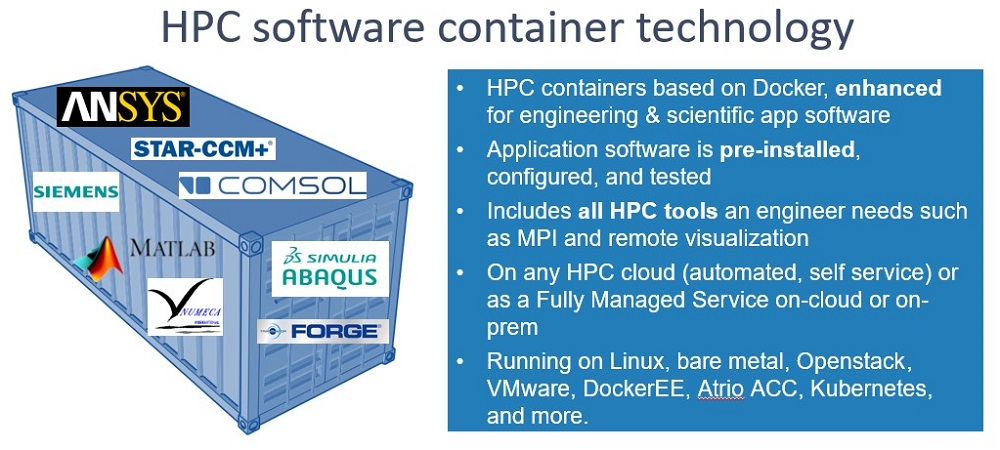
\includegraphics[scale=0.5]{./imgs/hpc-container.jpg}
	\captionsource{The container technology for HPC}{https://www.hpcwire.com/2019/09/19/kubernetes-containers-and-hpc/}
	\label{fig:hpc-container}
\end{figure}

Despite all those advantages, Kubernetes is not ready yet to be used in proper
HPC environment because it lacks vital components like a proper batch job
queuing system, and support for MPI applications. It cannot yet compete against
the very well established HPC ecosystem, but that time may come soon as
containers are becoming more and more integrated in modern infrastructures.

\section{Objectives}

The goal of this project is to design and implement Batkube, which will be an
interface between Batsim and Kubernetes schedulers. With this interface, we
want to compare Batsim results gainst data from a real Kubernetes cluster,
given HPC workloads.

\section{Technical challenges}
\subsection{Translation}
\subsection{Time hijack}
TODO

\SetKwInput{KwInput}{Input}
\SetKwInput{KwOutput}{Output}


\begin{algorithm}[H]
\DontPrintSemicolon
\KwInput{req: request channel, res: result channel map}
\While{Batkube is not ready} {
	wait\;
}
requests = []request\;
\While{req is not empty} {
	m = $<$- req \tcc{Non blocking receive}
	requests = append(requests, m)\;
}
sendToBatkube(requests) \tcc{Only requests with duration > 0 are actually sent. Batkube will always anwser.}
now = responseFromBatkube()\;
\For{m in range requests} {
	res[m.id] $<$-now \tcc{The caller continues execution upon reception}
}

	
\caption{Requester loop}
\label{alg:reqLoop}
\end{algorithm}


\begin{algorithm}[H]
\DontPrintSemicolon
\KwResult{Current simulation time}
\KwInput{d: timer duration, req: request channel, res: response channel map}
\KwOutput{now : simulation time}

\If{requester loop is not running}{
	go runRequesterLoop() \tcc{There can on ly be one loop runing at a time}
}
id = newUUID()\;
m = newRequestMessage(d, id) \tcc{Requests are identified using uuids}
resChannel = newChannel()\;
res[id] = resChannel \tcc{A channel is associated with each request}
req $<$- m \tcc{The code blocks here until request is handled}
now = $<$-resChannel \tcc{The code blocks here until response is sent by the requester loop}
return now\;
\caption{Time request (time.now())}
\label{alg:now}
\end{algorithm}


\subsection{Time synchronisation}

\begin{algorithm}[H]
	\caption{Synchronisation with timers}
	\label{alg:sync_timers}
	\DontPrintSemicolon
	\KwInput{timeout: time.Duration; simulationTimestep: time.Duration}

	stopWaitingForMessages := false\;
	\While{!stopWaitingForMessages}{
		getTimerRequests() \tcc{Translate timers requested by the scheduler to CALL\_ME\_LATER events}
		getSchedulerDecisions() \tcc{Translate scheduler decisions to Batsim messages}
		\If{decisionReceived() or timeSinceLastMessage() > timeout}{
			stopWaitingForMessages = true
		}
	}
	\tcc{We keep track of all REQUESTED\_CALL events yet to come}
	\If{durationToNextRequestedCall > simulationTimestep}{
		addCallMeLater() \tcc{Add a CALL\_ME\_LATER event with timestamp now + simulationTimestep
		}
	}
\end{algorithm}

\bigskip

\begin{algorithm}[H]
	\caption{Synchronisation with incremental time increases}
	\label{alg:sync_timers}
	\DontPrintSemicolon
	\KwInput{simulationTimeout: time.Duration; incrementTimeStep: time.Duration; incrementValue: time.Duration}

	stopWaitingForMessages := false\;
	incremented := 0\;
	\While{!stopWaitingForMessages}{
		getSchedulerDecisions()\;
		\If{decisionReceived() or incremented >= simulationTimeout}{
			stopWaitingForMessages = true
		}\ElseIf{timeSinceLastIncrement() > incrementTimeStep}{
			\tcc{this last condition is here to slow down this process and give time for the scheduler to take its decisions}
			now = now + incrementValue\;
			incremented = incremented + incrementValue
		}
	}
	addCallMeLater() \tcc{Add a CALL\_ME\_LATER event with timestamp now + incrementValue}
\end{algorithm}

\subsection{Re-building the API}

\chapter{Evaluation}

\chapter{Conclusion}


\backmatter
\printbibliography
\end{document}
